\documentclass[12pt]{article}

\usepackage{sbc-template}

\usepackage{graphicx,url}

%\usepackage[brazil]{babel}   
\usepackage[utf8]{inputenc}  

     
\sloppy

\title{Algoritmos II\\ Trabalho Prático II}

\author{Rodrigo S. Nascimento\inst{1} \\2021067534}

\address{DCC -- Universidade Federal de Minas Gerais
  (UFMG)\\
  Belo Horizonte -- MG -- Brasil
}

\begin{document} 

\maketitle

\begin{abstract}
  This paper addresses the practical aspects of algorithms used to solve NP-hard problems, with a focus on evaluating implementations for computing routes in the Traveling Salesman Problem (TSP). The analysis presented focuses on an exact solution based on Branch-And-Bound, in addition to two approximate solutions known as Twice-Around-The-Tree and Christofides algorithm, applied to the Euclidean TSP.
\end{abstract}
     
\begin{resumo} 
  Este artigo aborda os aspectos práticos dos algoritmos utilizados na resolução de problemas difíceis, com foco na avaliação de implementações para a computação de rotas no Problema do Caixeiro Viajante ou Traveling Salesman Problem (TSP). A análise apresentada concentra-se em uma solução exata baseada em Branch-And-Bound, além de duas soluções aproximadas conhecidas como Twice-Around-The-Tree e algoritmo de Christofides, aplicadas ao TSP euclidiano.
\end{resumo}


\section{Introdução}

O Problema do Caixeiro Viajante (TSP) representa um desafio fundamental em otimização combinatória, onde o objetivo é encontrar a rota mais eficiente que permita a um viajante visitar todas as cidades em um conjunto dado, retornando ao ponto de origem. Dada a natureza NP-difícil do problema, a busca por soluções eficazes torna-se uma tarefa complexa. Neste contexto, o presente artigo propõe explorar aspectos práticos relacionados à implementação de algoritmos para resolver o TSP. Três abordagens específicas foram exploradas: uma solução exata baseada em \textbf{Branch-And-Bound}, e duas soluções aproximadas - algoritmo \textbf{Twice-Around-The-Tree} e o algoritmo de \textbf{Christofides}. Baseando-se em um conjunto de dados com número variado de cidades para o problema em questão, todos os algoritmos foram submetidos a avaliação de três métricas de execução: qualidade da solução, tempo e espaço.

\section{Implementação} \label{sec:firstpage}

As implementações dos algoritmos foram inteiramente desenvolvidas na linguagem Python versão 3.10.8. Especificações do ambiente de desenvolvimento: Sistema operacional Windows 10 com uso do recurso Windows Subsystem for Linux (WSL) na distribuição Ubuntu, Processador AMD Ryzen 7, 8GB de memória RAM.

\subsection{Instâncias do TSP}

Todas as instâncias do TSP utilizadas nas execuções dos algoritmos correspondem a grafos completos obtidos da transformação de um conjunto de cidades de um banco de dados com auxílio da biblioteca networkx. Mais detalhes sobre os dados usados serão discutidos na sessão de experimentos. Assim, as cidades são representadas por vértices e o caminho entre elas são arestas com seus respectivos pesos que correspondem a distância entre cidades. A escolha da utilização de grafos como estrutura de dados para representar cidades no problema do caixeiro viajante já é bastante estabelecido uma vez que facilita a implementação de soluções conforme mostrado nos itens seguintes.

\subsection{Branch-And-Bound (BNB)}

A solução BNB é exata, ou seja, encontra o custo ótimo do percurso para o TSP e apresenta uma complexidade exponencial. Dentre todas as abordagens exploradas neste artigo, o algoritmo implementado para o BNB foi o mais complexo e que exigiu mais escolhas de implementações para driblar dificuldades. A essência dos algoritmos Branch-And-Bound reside na exploração de todas as possibilidades em uma árvore de decisões, utilizando como critério para a próxima etapa da busca uma estimativa "otimizadora" do custo associado a um determinado ramo. Uma vez que um caminho é concluído, ele se torna a melhor solução até o momento, e caminhos com estimativas mais desfavoráveis são "podados" e não são mais investigados. Esse descarte de caminhos pode resultar em uma significativa redução no espaço de busca.

Para a implementação do BNB, o primeiro passo foi definir a classe Node que agrupa cada nó na exploração do algoritmo e apresenta um método de comparação entre eles. O principal desafio para o uso do BNB no problema TSP é estabelecer uma função Bound de estimativa que seja rápida. Nesta implementação, uma estimativa inicial do custo ideal de um circuito hamiltoniano, implementada na função \texttt{initial\_bound()}, é feita em tempo polinomial quadrático baseando-se nas duas arestas de menores pesos que saem de cada vértice. Para cada nó da árvore de busca, o custo é atualizado na função \texttt{update\_bound()}. Como apenas um vértice é inserido a cada nó, então é adicionada apenas uma aresta por vez. Dois casos são considerados: se a aresta inserida é uma das menores para aquele vértice do grafo ou outro. Se a aresta inserida é a primeira para o nó analisado mas não é menor para este, então o custo deve ser atualizado pela diferença de peso entre a maior das menores e a aresta inserida, pegando o teto da divisão por 2 desse incremento. Foi utilizado um marcador booleano para indicar se já foi inserida uma aresta naquele nó ou não. A lógica para os demais casos é a mesma. 

A implementação da função Bound é a parte mais complexa do algoritmo. Após sua funcionalidade estabelecida, na primeira vez que um caminho é completamente percorrido na árvore de busca, o nó folha passa a ser uma solução candidata. As estimativas são comparadas com o custo da solução candidata e são percorridas mais profundamente se tiverem potencial de superação, atualizando a solução candidata caso necessário.

\subsection{Twice-Around-The-Tree (TATT)}

O algoritmo de implementação mais simples entre as soluções exploradas. Através do uso da biblioteca networkx para o cálculo da árvore geradora e para o percurso pré-ordem dos vértices, este algoritmo, que possui um fator de aproximação de 2, tem como ideia principal a exploração de árvores geradoras mínimas (AGM). A simplicidade computacional está na facilidade de calcular a AGM e o ciclo encontrado pelo algoritmo, sendo este, no máximo, duas vezes pior que o ciclo ótimo. Após obter a AGM, o grafo é percorrido utilizando uma DFS para construir o caminho, excluindo repetições. O último passo é calcular o custo do ciclo final através de um laço simples sobre suas arestas. A complexidade do algoritmo é dominada pela computação da árvore geradora mínima.

\subsection{Christofides}

O algoritmo de Christofides é uma abordagem de fator aproximativo ainda mais eficiente (1.5 comparado ao custo ótimo) para o Problema do Caixeiro Viajante (TSP) e também mais complexa. Assim como no algoritmo TATT, a primeira etapa envolve a construção de uma árvore geradora mínima do grafo original. A ideia principal é caminhar o circuito euleriano, transformando-o em hamiltoniano. Na implementação dessa etapa, foi feito um matching perfeito de peso mínimo em um subgrafo induzido pelos vértices de grau ímpar. Um multigrafo resultante das arestas do matching e da AGM foi usado para o cálculo do circuito euleriano. Excluindo os vértices repetidos, chega-se a uma lista de vértices que corresponde ao circuito hamiltoniano desejado. Todos esses passos foram feitos com o auxílio de funções disponíveis na biblioteca networkx. Por fim, foi calculado o custo total do circuito obtido. A complexidade do algoritmo é dominada pela computação do matching de peso mínimo.

\section{Experimentos}

Como conjunto de teste, foram utilizadas instâncias compiladas na biblioteca TSPLIB conforme especificado nas instruções do trabalho prático. Em particular, foram consideradas apenas as instâncias cuja função de custo seja a distância euclidiana em 2D. Dessa forma, os pesos das arestas dos grafos completos gerados do conjunto de dados foram estabelecidos com as distâncias euclidianas entre os pontos 2D que correspondem às cidades. Ao todo, 78 conjuntos de dados para o problema TSP foram utilizados para os experimentos, cada conjunto possui um limiar que indica a solução ótima do problema. O menor conjunto possui 51 cidades e o maior possui 18512 cidades. Todos os conjuntos foram processados por cada um dos algoritmos apresentados no item anterior com a coleta de 3 métricas de desempenho: qualidade da solução, tempo de execução e uso de memória. 

Para obter a qualidade da solução, foi considerado o cálculo do fator de aproximação entre a solução encontrada pelo algoritmo e a solução ótima dada pelo limiar de cada conjunto. Na coleta do tempo de execução, foi utilizada a biblioteca time padrão de Python para obter a diferença entre o tempo de início e fim da execução de cada algoritmo no processamento das instâncias. Por último, a quantidade de memória (em megabytes) usada por cada algoritmo durante a execução foi obtida através da biblioteca memory profiler. A execução de cada algoritmo foi limitada a um tempo máximo de 30 minutos para validar uma coleta de dados.

\section{Resultados}

\subsection{Limitações}

Todos os experimentos realizados com o algoritmo Branch-And-Bound apresentaram um tempo de execução superior a 30 minutos. Isso significa que, para as instâncias presentes no conjunto de testes, não é possível encontrar o valor ótimo do circuito entre as cidades em um tempo hábil. Esse resultado revela que, embora os algoritmos BNB possuam estratégias para otimizar a busca, como a eliminação de soluções inviáveis, a complexidade intrínseca desses problemas combinatórios pode resultar em uma execução mais demorada. De fato, a complexidade computacional continua sendo exponencial e mesmo que as instâncias sejam pequenas o tempo de execução pode ser longo. Dessa forma, a coleta de métricas de avaliação não foi possível para a implementação aplicada.

Para os algoritmos aproximativos Twice-Around-The-Tree e Christofides, 70/78 dos conjuntos de teste para os experimentos foram bem sucedidos na coleta de métricas. As instâncias de maior tamanho (a partir de 4000 cidades) receberam um aviso de falha de memória durante a execução. O provável motivo dessa falha é a deficiência de recursos computacionais no ambiente de execução pelo uso do Windows Subsystem for Linux (WSL). Apesar dessa limitação, dados suficientes foram coletados para uma avaliação de desempenho das soluções aproximadas.

\subsection{Tempo de Execução}

A Figura 1 mostra a relação entre o número de cidades das instâncias do TSP com os tempos de execução dos algoritmos aproximativos. É possível observar que o algoritmo TATT apresentou tempos consideravelmente inferiores ao algoritmo de Christofides. Esse resultado era esperado devido a complexidade assintótica do TATT ser limitada pela construção da árvore geradora mínima, o que é feito em O(m log n) onde m é o número de arestas e n é o número de vértices do grafo. 

Por outro lado, a complexidade do algoritmo de Christofides é dominada pela computação do matching de peso mínimo, que é da ordem de O(n3) onde n é o número de vértices do grafo. Dessa forma, conforme o número de cidades aumenta, a curva do tempo de execução de Christofides tem uma taxa de crescimento mais elevada que o TATT. Nenhuma instância demorou mais que 17 minutos para ser computada.

\begin{figure}[h]
\centering
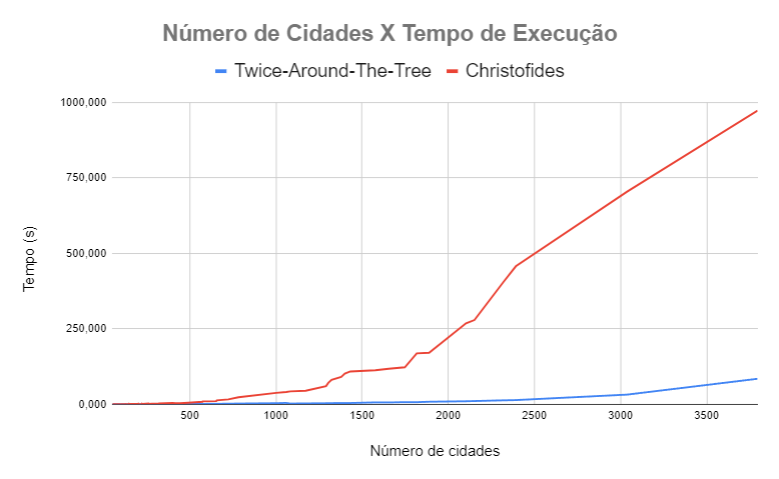
\includegraphics[width=\textwidth]{Time.png}
\caption{Número de Cidades vs Tempo de Execução para os algoritmos aproximativos.}
\label{fig:time}
\end{figure}

\subsection{Uso de memória}

O algoritmo TATT demonstrou demandar uma quantidade ligeiramente menor de memória em comparação com o algoritmo Christofides conforme observado na Figura 2. Essa observação pode ser atribuída à abordagem simplificada que ele utiliza. Por exigir menos operações complexas, esse algoritmo pode ser mais eficiente no que diz respeito ao consumo de memória. 

Já o algoritmo Christofides, que incorpora estratégias mais elaboradas, demanda recursos adicionais de memória. As operações mais intrincadas realizadas pelo algoritmo podem resultar em uma alocação maior de memória durante a execução. Portanto, o resultado encontrado está dentro do esperado. Apesar da diferença ser mínima, é esperado que o Christofides permaneça mais tempo no estado de constância no consumo máximo de memória apresentado devido a sua implementação ser mais complexa. O maior consumo de memória observado foi 3346 megabytes para a instância do TSP com 3795 cidades.

\begin{figure}[ht]
\centering
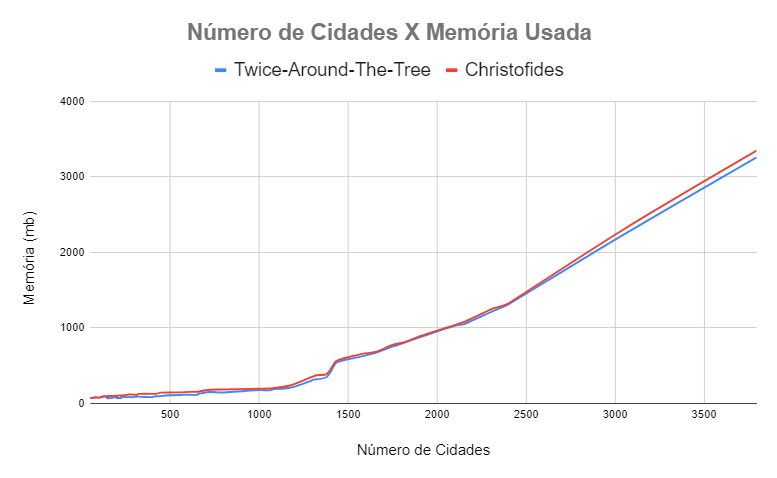
\includegraphics[width=\textwidth]{Memory.png}
\caption{Número de Cidades vs Memória Usada para os algoritmos aproximativos.}
\label{fig:memory}
\end{figure}

\subsection{Qualidade da Solução}

Embora o TATT compense significativamente em termos de tempo, a qualidade do ciclo encontrado pode ser insatisfatória. O algoritmo de Christofides, por outro lado, consistentemente resulta em custos menores conforme mostrado na Figura 3. Essa disparidade está de acordo com as expectativas, considerando que o algoritmo de Christofides tem um teto de fator de aproximação 1.5 vezes em relação ao ótimo, enquanto o TATT é aproximadamente 2 vezes. Nenhum experimento fugiu dos fatores de aproximação esperados e isso é um indicativo de que as implementações funcionam corretamente para as instâncias do TSP que foram computadas independente da quantidade de cidades.

A média dos fatores de aproximação corresponde a 1.37 e 1.12 para o TATT e Chrstitofides, respectivamente. Pode-se constatar que esses valores ficaram abaixo dos tetos de cada algoritmo. No caso do Christofides, as soluções encontradas estão muito próximas do valor ótimo e o algoritmo se torna uma boa escolha se desejado resultados mais precisos. O TATT também se torna uma boa opção para resultados mais rápidos.  

\begin{figure}[ht]
\centering
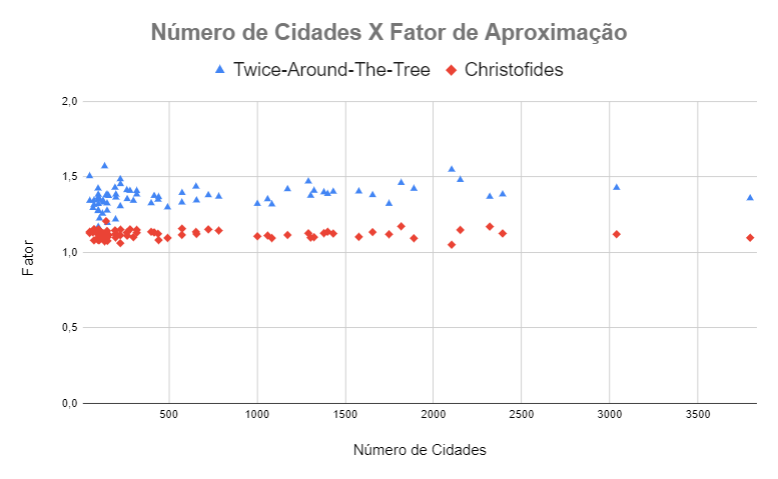
\includegraphics[width=\textwidth]{Quality.png}
\caption{Número de Cidades vs Fator de Aproximação referente a solução ótima para os algoritmos aproximativos.}
\label{fig:quality}
\end{figure}

\subsection{Considerações Finais}

Todas as métricas obtidas durante os experimentos se encontram em uma tabela disponível no arquivo "resultados.csv". As análises e gráficos apresentados nos itens anteriores se baseiam nos valores tabelados. O ideal seria uma repetição dos experimentos para se ter uma estimativa mais precisa com um valor médio de cada métrica, mas devido ao tempo longo para processar todos os conjuntos de dados, não se tornou viável esse feito.


\section{Conclusão}

A comparação entre algoritmos aproximativos e exatos para a resolução de problemas difíceis revelou nuances significativas em suas abordagens e desempenhos. Os algoritmos aproximativos, como o Twice-Around-The-Tree e o Christofides para o Problema do Caixeiro Viajante, destacam-se pela eficiência temporal, oferecendo soluções aceitáveis em um tempo de computação hábil para a grande maioria dos experimentos. Ficou evidente que as soluções aproximadas podem ser muito úteis visando eficiência no uso de recursos e ainda assim mantendo um compromisso de precisão aceitável diante ao valor ótimo.

Por outro lado, os algoritmos exatos, exemplificados pelo método de Branch-and-Bound, garantem a solução ótima mas com um custo de recursos que pode ser inviável na grande maioria dos casos, especialmente para problemas com dimensões consideráveis, devido a sua complexidade computacional.

Portanto, o trabalho prático evidencia as particularidades dessas abordagens e que a escolha deve ser cuidadosamente ponderada, levando em conta os requisitos específicos do problema em questão, bem como as restrições do ambiente de execução e o equilíbrio entre tempo e precisão desejados.

\section{Referências}

Goodrich, M. T., Tamassia, R. Algorithm Design and Applications. Editora Wiley, 1ª Edição (2015).

\end{document}
